\chapter{Réalité Augmentée}

  \section*{Vue Personnalisée}
  
    \paragraph{}
    Pour pouvoir afficher les icônes sur la caméra, il fallait dans un premier temps pourvoir gérer l'ouverture et la fermeture de celle-çi. Pour cela 
    nous avons dû avoir recours à une vue personnalisée. La vue personnalisée récupère les paramètres de la caméra du mobile, elle créée une surface que
    l'on va pourvoir utiliser dans nos layouts en mettant le chemin de notre classe.
    
    \end{onehalfspace}
    \begin{lstlisting}
<com.example.eyeway.realiteAugmente.CustomCameraView
        android:id="@+id/camera"
        android:layout_width="wrap_content"
        android:layout_height="wrap_content" />
    \end{lstlisting}
     \begin{onehalfspace}
  \section*{Positionner les points d'intérêt}
    
    \paragraph{}
    
    Le second travail est l'un des plus important de la partie réalité augmentée, il s'agit du positionement des points d'intérêt sur la caméra. Nous devons 
    pour cela récupèrer la position actuelle de l'utilisateur et la position du point d'intérêt. Nous faisons ensuite un calcul d'angle en récupèrant 
    l'angle entre nous et le nord ainsi que celui entre nous et le point d'intérêt. Ceci va nous permettre de savoir en fonction de l'orientation du téléphone
    , les points d'intérêt se trouvant dans la direction regardée par l'utilisateur.
    
    \paragraph{}
    Pour récupèrer notre position actuelle nous avons accès à deux ressources, le GPS  et le réseau du téléphone. Chacune de ces ressources comportent
    ses inconvénients et ses avantages. Le GPS a l'avantage d'être précis mais il a pour inconvénient d'être lent à se mettre en route dans certains cas
    d'utilisations, par exemple dans un bâtiment. Le réseau lui est plûtot rapide mais il comporte une marge d'erreur vraiment importante. 
    
    \paragraph{}
    Nous avertissons donc l'utilisateur lorsque le GPS n'est pas activé, en lui indiquant que sans l'utilisation de celui-çi l'application sera moins précise. Nous 
    avons donc absolument besoin de l'un ou de l'autre, c'est pourquoi nous bloquons l'utilisation de la géocalisation si l'itinérance de données n'est
    pas activée ou au moins une des deux ressources n'est pas activée.
    
    
    \paragraph{}
    L'étape suivante pour le positionement d'un point d'intérêt était de savoir en fonction de l'angle où le postionner sur l'écran. Pour cela nous 
    avons utilisé l'attribut margin pour placer l'imageView sur l'écran, nous récupèrons ainsi la hauteur, la largeur de l'écran, les valeurs renvoyées
    par l'accélérometre du téléphone et nous utilisons un calcul trouvé sur internet qui permet à partir de ces valeurs de connaître la position du point d'intérêt
    sur l'écran.
    
    \paragraph{}
    Chaque point d'intérêt aura une icône en relation avec son type de batîments et un label qui correspondra à la distance entre la position actuelle 
    de l'utilisateur. Nous devons donc pour chaque point d'intérêt recalculer le label lorsque la position de l'utilisateur change. Nous avons mis une
    icône par défaut si le type de batîment n'est pas connu.
    
    
    \section*{Création d'un nouveau point d'intérêt}

    \paragraph{}
    L'utilisateur peut à tout moment vouloir créer un nouveau point d'intérêt s'il le souhaite. Pour cela il devra appuyé quelques secondes sur l'écran,
    nous offrons la possibilité à l'utilisateur de renseigner certains champs : le nom, une description, l'adresse, le numéro de téléphone et le site 
    web de son nouveau point.
    
    \paragraph{}
    Nous pré-remplissons le champ adresse à l'aide de la classe GeoCoder qui permet de retourner en fonction d'une longitude
    et d'une lattitude l'adresse correspondante. L'utilisateur doit ensuite appuyé sur le bouton sauvegarder, ceci aura comme action de sauvegarder le 
    nouveau point comme favoris et de l'ajouter directement à l'écran. L'utilisateur pourra ensuite retrouver son nouveau point à chaque utilisation 
    de l'application dans le menu de gestion de favoris.
    
    \begin{center}
	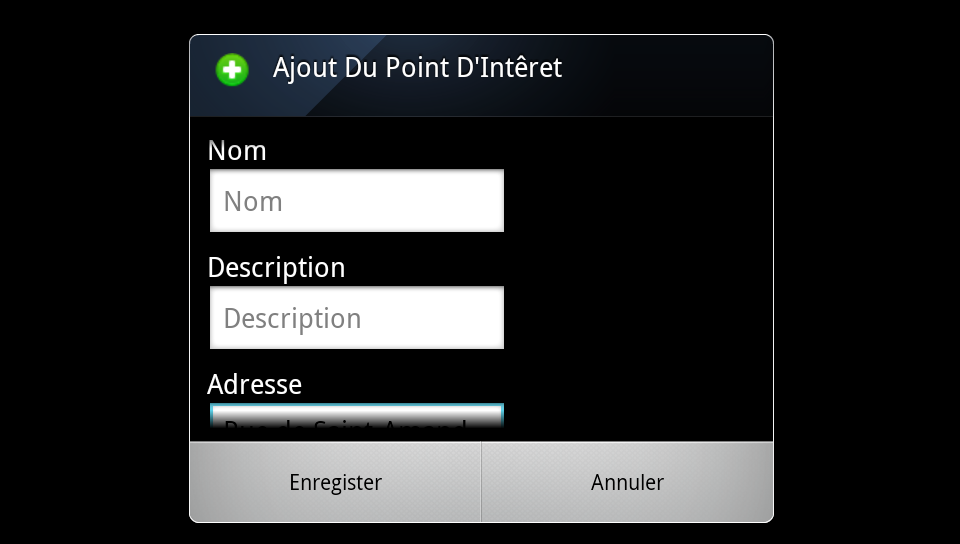
\includegraphics[width=140mm]{images/ajout_poi.png}
    \end{center}

      
    \section*{Détails d'un point d'intêret}
    
    \paragraph{}
    Pour avoir accès au détails d'un point d'intérêt, nous avons fait en sorte que les images soit cliquables. Donc lorsque l'utilisateur voudra le
    détails d'un certain point il devra juste cliquer sur l'icône en question. Lorsque le clic est effectué nous utilisons la requête de détails qui 
    va récupèrer le lieu complété avec les informations manquantes.
    
    \paragraph{}
    Une fois la requête executée nous affichons une boite de dialogue comportant tout les champs renseignés dans lieu. Et nous offrons aussi la possibilité
    à l'utilisateur de sauvegarder le lieu en question et de basculer vers la vue map pour calculer un itinéraire. La partie Map n'étant pas fonctionnelle
    nous avons pas eu la possibilité de l'utiliser.
    
    \begin{center}
	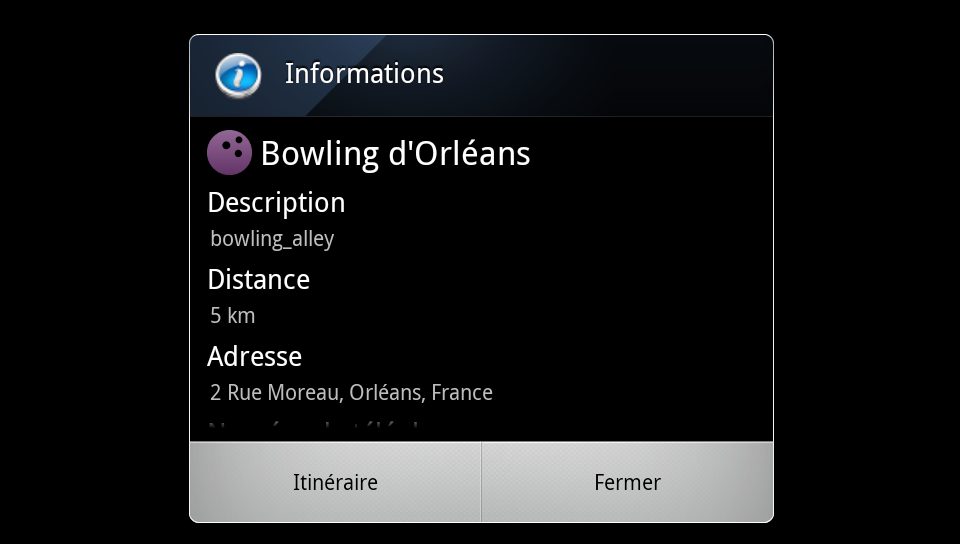
\includegraphics[width=140mm]{images/detail_poi.png}
    \end{center}
    
    \section*{Amélioration possible}
    
    \paragraph{}
    Pour la réalité augmentée nous aurions aimé pouvoir implémenter un systéme de guidage vers un point d'intérêt sélectionné par l'utilisateur. Pour 
    cela nous avions penser à utiliser une fléche qui dirigerais l'utilisateur vers sa destination.